\chapter{Introduction}  \label{chp_intro}
\section{Background}
% history of 802.11
Wireless local area networking (WLAN) has experienced tremendous growth in the last two decades with the proliferation of IEEE 802.11 devices. 
WLAN liberates people from fixed cable so that they could access to the world anywhere and anytime. 
IEEE 802.11 standardizes one type of WLAN on ISM band, which is free for commercial use from 1985. 
The first version of the 802.11 standard was ratified in 1997.
As a member of the IEEE 802.11 family of local area networking (LAN) and metropolitan area networking (MAN) standards, 802.11 interfaces with 802.1 architecture, management, and interworking, and 802.1 logical link control (LLC). 
The combination of 802.2 LLC and 802.11 MAC and PHY make up the data link and physical layers of the Open Systems Interconnection (OSI) reference model\cite{osi}.
The IEEE 802.11 working group began development of a common medium access control (MAC) layer for multiple physical layers (PHY) to standardize WLAN \cite{802.11spec}.
To interoperate between IEEE 802.11 devices from different manufacturers, the Wi-Fi Alliance (WFA)\cite{wifialliance} was formed in 1999 to certify interoperability by rigorous testing.

\begin{figure}[!h]
\begin{subfigure}[t]{.5\textwidth}  
\centering
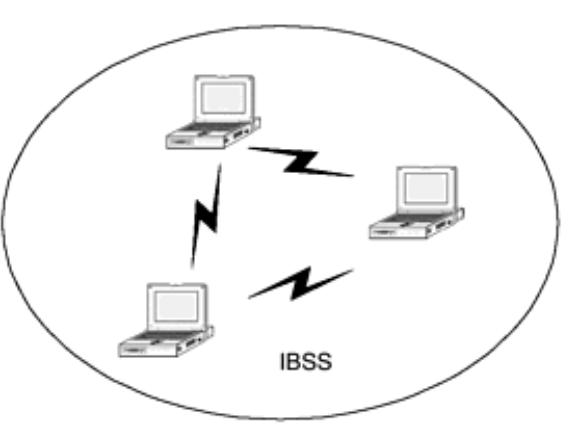
\includegraphics[scale=.3]{./figure/chp1/ibss.png}
\caption{Ad hoc mode}
\label{fig_adhoc}
\end{subfigure}
~
\begin{subfigure}[t]{.5\textwidth}  
\centering
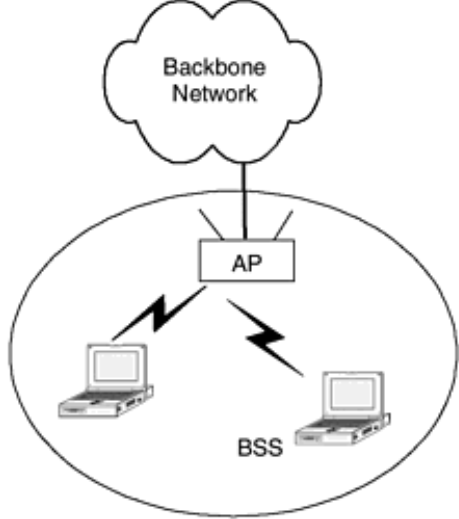
\includegraphics[scale=.3]{./figure/chp1/bss.png}
\caption{Infrastructure mode}
\end{subfigure}
\caption{Working mode of WiFi}
\label{fig_infras}
\end{figure}

WiFi has two working modes. 
The most common mode is infrastructure mode. The WLAN in such mode is called Basic Service Set (BSS), consist of one access point (AP) and multiple stations (STA) as Figure \ref{fig_infras} forming a star topology.
That means stations could only communicate with AP instead of communicate with each other directly. 
And we call the direction from AP to stations down-link (DL) and from stations to AP up-link (UL).
The other mode is Ad hoc mode, and the corresponding WLAN is called Independent BSS (IBSS) as Figure \ref{fig_adhoc}.
In the IBSS, all stations are equal and they could communicate directly only if the two stations could detect each other.
Our concern is the infrastructure mode.

The original (1997) 802.11 standard included three PHYs: infrared (IR), 2.4 GHz frequency hopped spread spectrum (FHSS), and 2.4 GHz direct requence spread spectrum (DSSS).
The DSSS data rates are 1, 2 Mbps.
This was followed by two standard amendments in 1999: 802.11b built upon enhanced DSSS with complementary code keying (CCK) to increase data rate to 11 Mbps in 2.4 GHz and 802.11a to create a new PHY in 5GHz to to increase data rate to 54 Mbps.
However, since the development of 802.11a introduced orthogonal frequency division multiplexing (ODFM) in 5 GHz, the adoption of 802.11a has been slow.
Subsequently, the 802.11 working group developed the 802.11g amendment, which incorporates the 802.11a OFDM PHY in the 2.4 GHz band.
What's more, 802.11g backward compatibility and interoperability is maintained between 802.11g and the older 802.11b devices.
% 802.11n
With the adoption of each new PHY, 802.11 has experienced a five-dold increase in data rate.
802.11n, called High Throughput Study Group (HTSG), improved data rate through the use of spatial multiplexing using Multiple-input and Multiple-output (MIMO)\cite{foschini1996layered} and 40 MHz operation.
A device equiped with multiple antennas may support at most 4 streams with MIMO. 
To take advantage of the much higher data rates provided by these techniques, MAC efficiency is also improved through the use of frame aggregation and enhancements to the block acknowledgment protocol.
% 802.11ac
Until 2013, to deal with increasing WLAN usage, a Very High Throughput (VHT) task group 802.11ac (TGac) was ratified, with even more streams and wider channel spacing.
Furthermore, a multi-user (MU) PHY, MU-MIMO\cite{bejarano2013ieee} was defined by the standard as a "technique where multiple stations, each with potentially multiple antennas, transmit and/or receive independent data streams simultaneously."\cite{802.11acspec}
That is, MU-MIMO allows stations having multiple antennas to transmit several data streams to multiple users at the same time over the same frequency channel.
This MU PHY is only MU on down-link (DL) transmission, from access point (AP) to station.

%\cite{802.11spec}, ac features\cite{bejarano2013ieee}, handbook \cite{o2005handbook}, 20billion shipment\cite{abiresearch}, \cite{wifialliance}, 

\begin{table}[!h]
\caption{Overview of 802.11 PHYs}
\centering
\label{table_PHY}
\begin{tabular}{p{2cm}p{1.8cm}p{1.8cm}p{1.8cm}p{1.8cm}p{2.8cm}}
\toprule  
   				& 802.11 	& 802.11b 	& 802.11g 	& 802.11n 	& 802.11ac \\
\hline
PHY technology	& DSSS		& DSSS-CCK	& OFDM/ DSSS & MIMO-OFDM	& MIMO-OFDM \\ 
\hline
Data rates		& 1,2 Mbps	& 5.5,11 Mbps& 1-54 Mbps& 6-600 Mbps& 6-1300 Mbps \\\hline
Frequency band	& 2.4 GHz	& 2.4 GHz	& 2.4/5 GHz	& 2.4/5 GHz & 2.4/5 GHz	\\\hline
Channel spacing	& 20 MHz	& 20 MHz	& 20 MHz	& 20,40 MHz& 20,40,80,160 and 80+80 MHz\\\hline
Maximum streams	& 1			& 1			& 1			& 4			& 8 \\ 
\bottomrule
\end{tabular}
\end{table}

% MAC CSMA/CA,
Influenced by the huge market success of Ethernet (standarded as IEEE 802.3), the 802.11 MAC adopts the same distributed access protocol, carrier sense multiple access (CSMA).
With CSMA, a station wishing to transmit first listens to the medium for a predetermined period, called dilivery inter-frame spacing (DIFS) in 802.11. 
If the medium is sensed to be "idle" during this period then the station is permitted to transmit. 
If the medium is sensed to be "busy", the station has to defer its transmission with a random period, called backoff counter in 802.11. The backoff counter is randomly generated among a contention window.
Then the the station will transmit until backoff counter decreases to zero.
And when a collision is detected, the contention window will double, which is called binary exponential backoff (BEB).
Since in radio communication, it's impossible for a station to detect a collision during its transmission.
A two-way handshake, which means each transmission requires an acknowledge, is used to determine whether the transmission is successful or not.
The acknowledge frame is responded after short IFS (SIFS), which equals time for receiving, processing the transmitted frame and generating an ACK frame.
Thus 802.11 uses a variation called CSMA/CA or CSMA with collision avoidance. 
With CSMA/CA, only if the station detects idle medium, the backoff counter will decrease.
Otherwise, it is frozen.
More details of DCF could be referred to \cite{802.11spec}.

Above is the foundation of MAC, which is called Distributed Coordination Function (DCF).
The simplicity of this distribtuted access protocol enables consistent implementation across all nodes, significantly contributed to Ethernet's rapid adoption as the industry LAN standard.


\begin{figure}[!t]
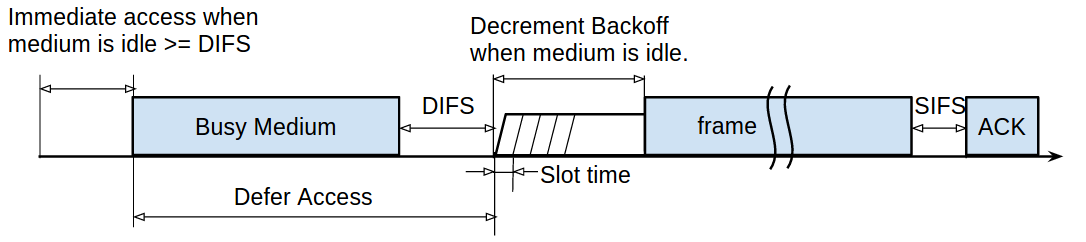
\includegraphics[scale=0.41]{./figure/chp1/dcf.png}
\caption{DCF working procedure}
\label{fig_dcf}
\end{figure}

\section{Challenge of WiFi}
% dense scenario
During last decades, IEEE 802.11 achieved great success in WLAN. Enormous WiFi are deployed for its high speed and simplicity of deployment. 
More and more people are inclined to using mobile devices to access the Internet.
According to Cisco Visual Network index\cite{cisco2016}, the mobile traffic will increase 53\% at CAGR within 2015-2020 reaching 30.6 EB per month by 2020, which means increase eight-fold during the 5 years.
WiFi as the most popular technique of WLAN are confronting an absolutely big challenge of dense scenario.
The dense scenarios, according to the TGax simulation scenario  \cite{802.11ax_simu} of 802.11ax, are various, such as enterprise building with dense deployment of BSS or indoor/outdoor hotspot with dense users etc.
Though the data rate of WiFi has surpassed Gbit/s, the quality of experience (QoE) \cite{qoe} is not improved with the PHY's growth.
Problems arise with more and more dense deployment of WiFi.
That is because the bottleneck is located at MAC, which is not efficient under such a dense scenario.
Though previous amendments have made some improvements especially in 802.11n including aggregation of packets together with block ACK mechanism, reduced IFS (RIFS) etc.
Something defects inherent are not modified or improved in legacy amendments.

This section will explain that the bottleneck of throughput is located at MAC. 
DCF, as the foundation of MAC, is not efficient under dense scenario.
We display clearly about two inherent defects of legacy 802.11 MAC, including instability of DCF and unfair queueing problem.

\subsection*{Instability of DCF}
Since DCF is a distributed access protocol, CSMA/CA could not avoid all collisions, especially under a real world BSS where hidden terminals and wireless loss exist.
Many works have discussed about the stability of Random access \cite{szpankowski1983packet}. 
One good solution RTS/CTS mechanism, which is a four-way handshake, helps mitigate the collision under dense scenario. 
However, since RTS/CTS protects data transmission with the cost of more control frame exchange overhead, it is often enabled when the packet length exceeds a threshold, default as 2346 bytes.

Bianchi has made a great saturated analysis of DCF in 2000 that stations are assumed with non-empty queue. 
The throughput of Bianchi's work is defined as fraction of time the channel is used to successfully transmit payload bits.
As in Figure \ref{fig_thp_legacy}, the throughput degrades sharply with the number of stations increasing .
We could extend Bianchi's analysis to obtain the energy performance.
Stations have roughly three working states, "transmit", "receive" and "idle".
Check the Figure \ref{fig_part_state}, with the number of stations increases, the partition of time working in transmit state for each station decreases a lot while partition in receive state increases much. 
That means a station has much less chance to transmit. And with the decrease throughput, we could know that most of transmissions are collided with others. 
Then let's look at the energy performance by checking the Figure \ref{fig_eng}. 
We find that total energy consumption of a station increase a lot while successful transmissions are less.
Most of energy are wasted on listening to collided transmissions.
We thus could conclude that the DCF is inherently unstable and is not fit for dense scenario.


\begin{figure}[!h]
\centering
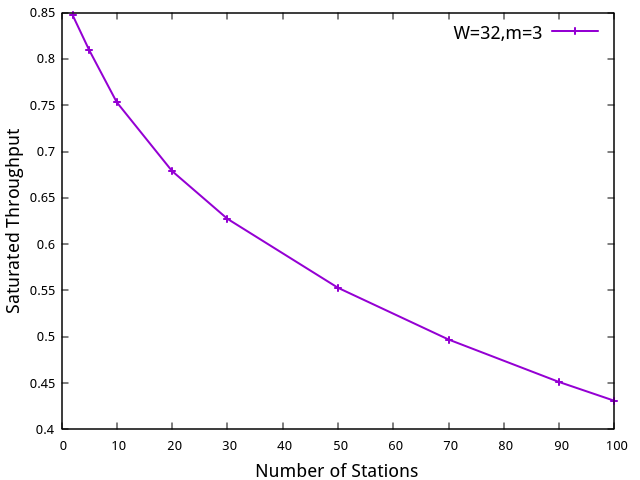
\includegraphics[scale=0.85]{./figure/chp1/n_throughput.png}
\caption{Saturated analysis: throughput vs number of stations}
\label{fig_thp_legacy}
\end{figure}
\vspace*{0.5cm}

\begin{figure}[!h]
\centering
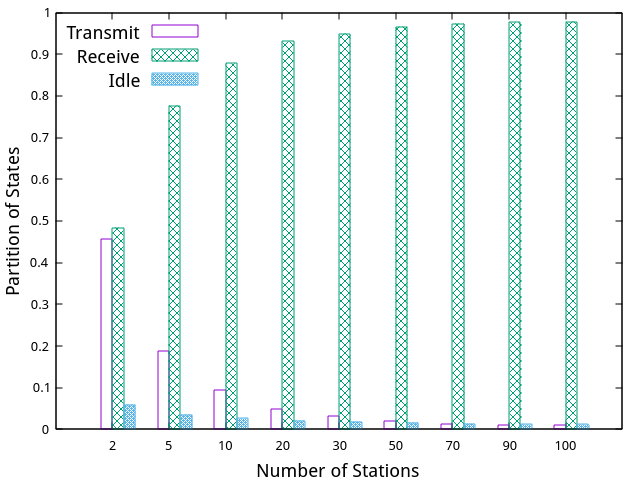
\includegraphics[scale=0.85]{./figure/chp1/n_state_partition.png}
\caption{Partition of working states of a station under saturated condition}
\label{fig_part_state}
\end{figure}

\begin{figure}[!h]
\centering
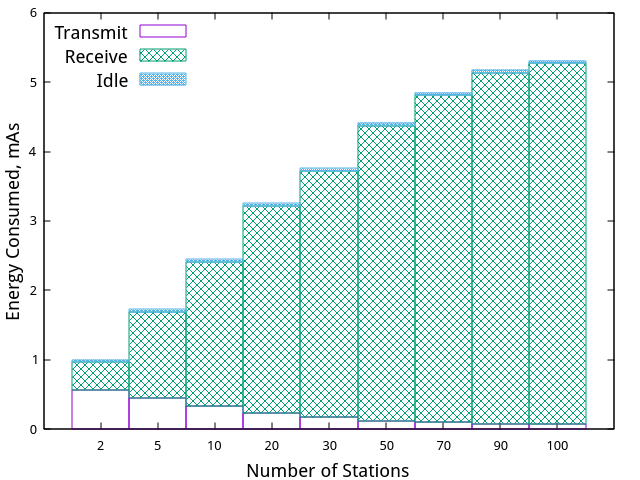
\includegraphics[scale=0.85]{./figure/chp1/n_energy_partition.png}
\caption{Energy consumption of a station under saturated condition}
\label{fig_eng}
\end{figure}

%With DCF, a random access MAC, the star topology of a 802.11 WLAN result in a absolutely unfair queueing. 
%Since in star topology,  access point (AP) needs to transmit all the down-link (DL) traffic, which is often more than $1/2$ traffic loading of the basic service set (BSS), while AP has only $1/n$ chance to access medium where $n$ is number of total stations including AP. It is, thus, an unfair queueing problem.
%What's worse, combining effect of the unstability of random access's nature and the unfair queueing problem, once under a dense scenario, the performance will degrade severely since contention and collision will occupy the channel.
%That lies the defect of legacy 802.11.
%We collectively call them dense deployment problem.
%The dense deployment problem not only degrades throughput but also waste much energy.

\subsection*{Unfair Queueing Problem}
%2. ax feature, MU, central control, but OFDMA-random access
DCF together with the star topology of a BSS results in a absolutely unfair queueing. 
Check the figure \ref{fig_unfair_queueing}.
When we see the BSS with queue model, each station will be a queue, including AP.
And channel is the server, which serve packets from stations. Channel capacity determines the serve rate.
Since BSS is star topology, access point (AP) needs to transmit all the down-link (DL) traffic, which means AP shares more than 1/2 traffic loading of a BSS. 
However, since DCF is a distributed random access mechanism, AP has only $1/n$ chance to access medium where $n$ is the number of total stations including AP. It is, thus, an unfair queueing problem for up-link (UL) and DL transmission. 
This problem may not lead to bad consequence only if the "server" is fast enough. 
That's what a list of previous amendments, like 802.11n and ac, were doing, improving throughput from 2 Mbit/s to 7 Gbit/s. 
However, this solution doesn't resolve the unfair queueing inherently. 
The unfair queueing is always there only if each station access channel with DCF.
Once the BSS becomes congested the unfair queueing will worsen the effect of instability of DCF, resulting in more waste of spectrum and energy.
\begin{figure}[!h]
\centering
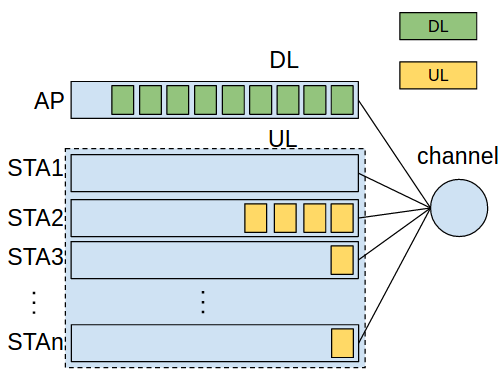
\includegraphics[scale=0.5]{./figure/chp1/unfair_queueing.png}
\caption{Unfair queueing problem of BSS}
\label{fig_unfair_queueing}
\end{figure}

\section{Solution: 802.11ax}
The TGax Project Authorization Request (PAR) \cite{802.11ax_par} states that "enable at least one mode of operation capable of supporting at least four times improvement in the average throughput per station in a dense scenario, while maintaining or improving the power efficiency per station."
To achieve the goal, the TGax would define standardized modifications to both the IEEE 802.11 physical layers (PHY) and the IEEE 802.11 Medium Access Control layer (MAC).

As stated in previous sections, previous amendments, like 802.11n and 802.11ac called high throughput (HT) and very high throughput (VHT) respectively, mainly focus on modifying PHY layer to improve data rate\cite{perahia2013next}. 
However, the real world WLAN suffers a lot from instability of DCF and unfair queueing problem under dense scenario. 
The bottleneck is located at the MAC layer.
Only if MAC is efficient, growth of PHY data rate could play a role in improving quality of experience (QoE) and energy efficiency.
Confronting the dense deployment scenario, 802.11ax introduces huge modifications to both PHY and MAC layers.

% PHY
First, an new MU PHY is created in 802.11ax, MU-OFDMA. 
As introduced in 802.11ac, MU-MIMO has realized MU PHY, which enables a station with multiple antennas transmit multiple streams to several stations.
However, it is only a DL MU.
The MU-OFDMA enables both DL and UL MU, while UL MU is more complicated since it is a transmission from $n$ stations to $1$ AP.
Thus, correspondingly see Figure \ref{fig_RU_spec}, a new control frame is created called Trigger Frame (TF) to initiate a MU UL transmission\cite{draft_ax}.

% MAC
Second, this TF-based MU UL permits AP as central controller to schedule both DL and UL transmission, which transfers the distributed access protocol to a centrolized access protocol. 
In this way, 802.11ax's MAC will not be a distributed random access mechanism and unfair queueing problem could be resolved inherently.
Actually, the new MAC is based on DCF since it helps co-exist among Overlap BSSs and other systems. 
The difference is that the DCF mainly works on AP which means AP needs to access channel following DCF procedure, while HE-STA (802.11ax STA) is scheduled by AP. 
The contention between AP and stations doesn't exist any more.


% random access
Though AP need not contend with stations, random access for non-AP stations are still necessary for its high efficient under light traffic scenarios.
Thus, under the new MU-OFDMA PHY, a multi-channel random access is also proposed in the 802.11ax standard draft \cite{draft_ax}. 
They could be an efficient way for stations to initiate a traffic stream by sending bandwidth request.
Different from DCF, the parameters like contention window are dynamically configured by AP.
MU PHY also adds complexity of the mechanism.
Detailed illustration of 802.11ax features is in chapter \ref{chp_ax_feature}.


\section{Related Work}
%3. related work, random acces history ? , clarify OFDMA-based random access is special
% SU/MU; aloha/CSMA; BEB/UB; saturated/unsaturated
Random access is one approach of multiaccess sharing in data network. 
It originates from Aloha and slotted Aloha in single-user channel\cite{abramson1970aloha}.
Random access is high efficient especially for short packets \cite{bertsekas1992data}.
Inherently, collision resolution algorithms can achieve small delay with a large number of lightly loaded nodes, the stability is a major concern\cite{bertsekas1992data}\cite{shen2003performance}. 
Then CSMA works as typical collision resolution  \cite{kleinrock1975packet}, which is modified then adopted by IEEE 802.11, named CSMA/CA. 

%\cite{chen1994medium}\cite{choi2006multichannel}\cite{cheng2013iterative} \cite{wei2012modeling}\cite{wu2013fasa}\cite{zhou2008efficient} \cite{paiva2011random} \cite{behroozi1992delay} \cite{ren1995transient}

With the emergence of MU PHY techniques, like MU-MIMO or MU-OFDMA, multi-channel random access is adopted by cellular networks.
They are normally designed for initial transmission access.
The multi-channel random access is Aloha-like access and has more requirement on synchonization. 
It is slowly developed in unlicensed band WLAN, such as WiFi, because of the complexity compared with simple DCF.
However, WiFi is now confronting the bottleneck of DCF, 802.11ax will adopt OFDMA to realize MU PHY.
The OFDMA-based random access in this thesis is also a Aloha-like access. 
Actually, a couple decades ago, some have been worked on this MU random access\cite{rubin1978group} \cite{tan1987performance}\cite{marsan1987multichannel}\cite{zhang1992multichannel}\cite{pountourakis1992analysis}\cite{birk1999judicious}.
In recent years, several analytical models have been proposed to derive the throughput \cite{zhou2008efficient} \cite{shen2003performance} \cite{choi2006multichannel}, the collision probability \cite{kim2012performance} \cite{seo2011design}, and the access delay \cite{zhou2008efficient}\cite{kim2012performance} \cite{seo2011design}\cite{behroozi1992delay}. 
In \cite{kim2012performance}, the authors presented an analytical model to evaluate the access success probability and the access delay for UMTS system.

The backoff mechanism determines the way of retransmission when failure occurs. 
Binary exponential backoff (BEB) is one of typical backoff mechanism, which has been applied by 802.11 until now.
The multi-channel Aloha-like access is always targetd for effective usage of multi-channel. 
\cite{choi2006multichannel} designs a 1-persistent type retransmission, i.e., no exponential backoff, to achieve a fast access.  
In \cite{zhou2008efficient}, a closed-form expression of throughput for OFDMA system is firstly given.
Many works compare performance of two backoff mechanism, binary exponential backoff and uniform backoff, like \cite{zhou2008efficient} \cite{seo2011design} \cite{kim2012performance}.
The two backoff mechanisms are implemented by IEEE 802.16 and 3GPP LTE respectively.  \cite{wei2015modeling} specifies a model estimating transient behavior of OFDMA system.

Most works are working on steady state behavior. The transient analysis of the slotted Aloha protocol was first presented in \cite{ren1995transient}. 
However, it is not clear how to  generalize the model to acccommodate multi-channel slotted Aloha systems with a time-varying retransmission probability due to backoff policy.
The random access with bursty traffic has been investigated in \cite{wei2012modeling} \cite{wu2013fasa}.

%many metrics: throughput, mean and variance of access delay, stability
All above works about OFDMA random access is an Aloha-type access in cellular network.
In addition, \cite{GeneralizedOFDMACSMACA} is one of few works for 802.11 WLAN, which generalizes CSMA/CA to OFDMA system for 802.11. 



\section{Motivation}
% why you want to do this work
As stated above, WiFi's data rate of PHY has reached an extraordinary high speed, while the MAC efficiency has gradually become the bottleneck of the total performance improvement because of the inherent instability and unfair queueing problem from the DCF and star topology BSS under dense scenario.
However, 802.11ax which is planned to be ratified in 2017 aimmed at high efficient WLAN (HEW), standardizing great motifications on both PHY and MAC layers. 
Among the modifications, OFDMA-based random access is one deserving our attention for research, which is the focus of this thesis. 
Though OFDMA and multi-channel random access have been employed by IEEE 802.16 and 3GPP LTE for a long time.
It is the first time for 802.11ax to realize OFDMA and OFDMA-based random access, which is a huge evolution for 802.11.
The OFDMA-based random access is an important part of revolutionary modifications in 802.11ax. 
OFDMA-based random access employs binary exponential backoff, MU PHY and Trigger-based MU UL.
It is much different from \cite{GeneralizedOFDMACSMACA}, since \cite{GeneralizedOFDMACSMACA} is a CSMA-like random access while OFDMA-based random access is an Aloha-like random access.
As far as we know, no performance analysis of IEEE 802.11ax OFDMA-based random access has been published. 
And since the OFDMA-based random access mechanism is more flexible and has more parameters, it's more meaningful to do performance analysis of the mechanism so that AP could configure proper parameters.

We know that \cite{bianchi2000performance} proposes an accurate Markov chain model for DCF, which is CSMA-like.
In this thesis, we show that how to extend the model to generate another Markov chain for 802.11ax to precisely depict steady state behavior of the OFDMA-based random access.
We assume stations are under saturated condition which means their queues are never empty.
The saturated analysis is based on the key assumption of constant and independent collision probability $p$ whatever the packet is retransmitted or not.
Simulation validates our model to be accurate.
Then, we estimate the maximum system efficiency and minimum access delay. 
And at last, we evaluate effects of every system parameter. 

\section{Organization}
The thesis is organized as follows. 
More explanations of 802.11ax features are given in section \ref{sec_MU}. In section \ref{sec_RA_illu}, a detailed illustration of OFDMA-based random access procedure is presented.
Chapter \ref{chp_sys_model} contains the system model and derivation of two metrics, including system efficiency and access delay. 
Simulation which helps validate the system model is presented in this chapter.
Then chapter \ref{chp_perf_eval} is the performance evaluation of optimal performance and checks the impact of system parameters on performance.
Chapter \ref{chp_conclu} remains the conclusion remark and future work.
